\documentclass{standalone}
\usepackage{tikz}
\usetikzlibrary{calc}
\usetikzlibrary{3d}
\tikzstyle{inarrow}=[->, >=stealth, shorten >=.03cm,line width=1.5]
\tikzstyle{outarrow}=[<-, >=stealth, shorten <=.03cm,line width=1.5]
\begin{document}
\newcommand*{\mt}[1]{\mathtt{#1}}
\rotatebox{0}{
\scalebox{1}{
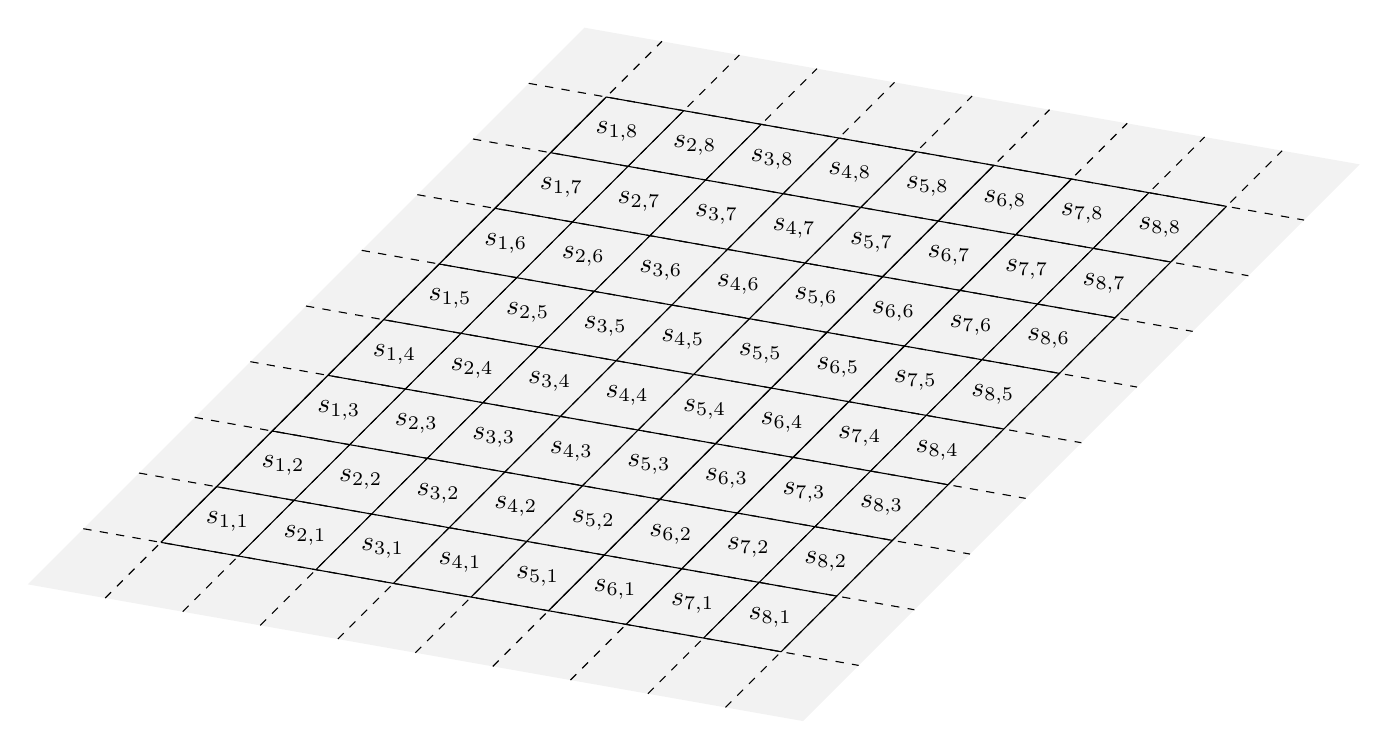
\begin{tikzpicture}[x={({cos(-10)*1cm},{sin(-10)*1cm})},y={({cos(45)*1cm},{sin(45)*1cm})},z={(0,1cm)}]
    \begin{scope}[canvas is xy plane at z=0]
        \fill[fill=gray!20, opacity=0.5] (0,0) rectangle (10,10);        
        \foreach \i in {1,...,9}{
            \draw[dashed] (0,\i) -- (10,\i);
            \draw[-] (1,\i) -- (9,\i);
        }
        \foreach \i in {1,...,9} {
            \draw[dashed] (\i,0) -- (\i,10);  
            \draw[-] (\i,1) -- (\i, 9);
            %\draw [very thin,gray] (\i,\yMin) -- (\i,\yMax)  node [below] at (\i,\yMin) {$\i$};
        }

        \begin{scope}[xshift=0.5cm, yshift=0.5cm]
            \foreach \i in {1,...,8} {
                \foreach \j in {1,...,8} {
                    \node at (\i,\j){$s_{\i,\j}$};   
                }
            }
        \end{scope}
    \end{scope}
\end{tikzpicture}}}
\end{document}